\chapter{Background \label{cha:chapter2}}

In order to set context of underlying thesis work, this chapter provides background information on virtualization technologies and embedded systems with special emphasis on the ARM platforms. A brief overview of Phidias, a static hypervisor in question is also given at the end of this chapter.

\section{Introduction to Virtualization \label{sec:tech}}
Virtualization is a mechanism of providing abstraction between computer hardware systems and softwares running on them, allowing us to create multiple computing environments exploiting the resource isolation on a single physical platform. It basically gives a logical view of multiple operating environments running on a single hardware. With the recent developments in virtualization, there has been huge investments in organizations over this technology to improve the efficiency and availability of resources and applications. Enterprises are giving up the old \textbf{one server, one application} model and gaining benefits from server consolidation provided by virtualization. Virtualization has dramatically changed the IT landscape by reducing its expenses and providing economies of scale and greater efficiency.

\subsection{History of Virtualization\label{sec:history}}
History of virtualization dates back to 1950's when the Compatible Time Sharing System (CTSS) was developed at MIT on IBM 704 series computer. The supervisor program of CTSS handled console I/O, scheduling of foreground and background (offline-initiated) jobs, temporary storage and recovery of programs during scheduled swapping, monitor of disk I/O, etc. The supervisor had direct control of all trap interrupts \cite{introtousevirtualization}.\\
\\
In the fall of 1963, MIT's Project MAC was founded with the main purpose of designing and implementation of a better time sharing system than CTSS. After IBM lost the bid to General Electric's GE 645, it created a number of virtual machine systems e.g, the CP-40 (developed for a modified version of IBM 360/40), the CP-67 (developed for the IBM 360/67), VM/370, and many more. We can roughly say that Virtual Machine technology was brought to users with the introduction of the CP-67 hypervisor on the S/360 Model 67 processor. In 1999, VMware introduced virtualization on x86 platforms. Since then, many vendos like Microsoft, Citrix etc had followed VMware and technology has been evolved with the advances in hardware architectures. 
\\
\\
\subsection{Benefits of Virtualization\label{sec:uses}}
For many years, server virtualization was considered one of the biggest advantages of using virtualization technology and VMware enjoyed a long run as king of x86 server virtualization. However, many players e.g. Citrix and Microsoft started to gain ground in this field by providing additional middleware and desktop virtualization offerings. Over the past several years, there has been huge deployments in virtualization and vendors are continuously innovating to increase virtualization capabilities of systems and developing management tools.\\
\\
There are many advantages of using virtualization technology. Following are some of the main benefits due to which virtualization has become a mainstream tool in the computing industry \cite{reasonstousevirtualization}:


\subsubsection{Better utilization of resources \label{sec:resource optimization}}
With virtual machines, resources of computing platforms can be used in an optimal manner to achieve better performance. Servers used in data centers typically have large resource capabilities. However, they are not fully utilized because of small number of connected users or less demanding applications. Virtualization of hardware allows on-demand resource allocation leading to efficient use of computing power, storage space and network bandwidth. In addition to on-demand usage of resources, virtualization also provides resource isolation between virtual machines. Each virtual machine can run software without affecting others code execution. 

\subsubsection{Consolidation \label{sec:Consolidation}}
For many years, individual servers have been dedicated to run single applications. For less demanding applications, computing capabilities would be wasted. With the advent of virtualization, organizations are now deploying several applications on single servers using only a small amount of processing power. Server consolidation has led to dramatic reduction in need of floor space, HVAC, A/C power, and co-location resources which has caused cost reduction and efficient power consumption.

\subsubsection{Security and Isolation\label{sec:security}}
Virtualization allows running multiple virtual machines in an isolated secure environment. All privileged calls made by guests' kernels are analyzed by hypervisor to provide safety against vulnerabilities and attacks. Exceptions and traps of one virtual machine are handled by hypervisor layer isolating other virtual machines from the resulting affects. Virtualization regulates access permissions to programs with reduced privileges from misusing resources. 

\subsubsection{Migration and Increased Uptime\label{sec:migration}}
Migration is the process of moving a running virtual machine from one place to another without affecting overall system. With virtualization, organizations can get better performance and reliable systems. It also increases uptime of servers and applications. Virtual machines can easily be backed up and restored for speedily recovery from computing disasters.


\subsection{Overview of Hypervisors\label{sec:aaa}}

A virtualization layer that separates the service request from underlying physical delivery of that request is called virtual machine monitor (VMM) or hypervisor. Hypervisor allows multiple operating systems to run concurrently within virtual machines on a single computer and provides dynamic allocation and sharing of physical resources e.g. CPU, memory, storage and I/O devices \cite{hypervisor1}.Hypervisor enables communication between hardware
and a virtual machine so that the virtualization accomplishes with this abstraction layer (hypervisor) \cite{hypervisor2}.  Figure \ref{Virtualization} shows the virtual machine abstraction architecture.

\begin{figure}[htb]
\centering
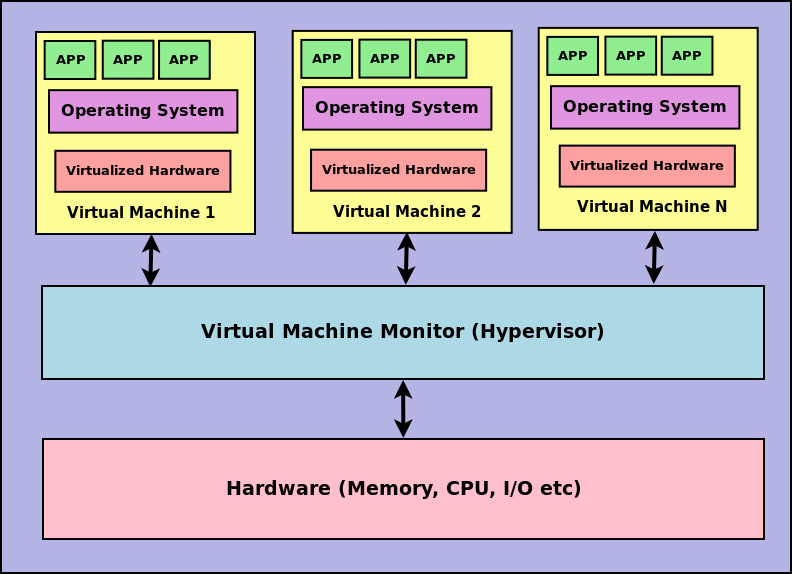
\includegraphics[width=10cm]{Virtualization_Abstraction}
\caption{Virtualization Framework}
\label{Virtualization}
\end{figure}
In 1974, Popek and Goldberg described the requirements of a hypervisor for efficient virtualization in the article `Formal Requirements for Virtualizable Third Generation Architectures' \cite{popek_goldberg_1973}. There are three requirements to be fulfilled by hypervisors:
\begin{itemize}
	\item Virtualization environment provided by hypervisor should be native system so that program behaves in a similar fashion.
	\item Virtualized resources should be shared with security controls to protect from any threats and performance interference.
	\item Good support to handle privileged instructions should be provided in order to avoid performace degradation.
\end{itemize}
Keeping in view the above requirements, different types of hypervisors have been introduced in market with different implementation level of virtualization which will be described in next sections.

\subsection{Types of Hypervisors\label{sec:bbb}}
There are two basic types of hypervisors i.e. Type 1 and Type 2 Hypervisors as shown in Figure \cite{Hyper1vsHyper2}.
\begin{figure}[htb]
	\centering
	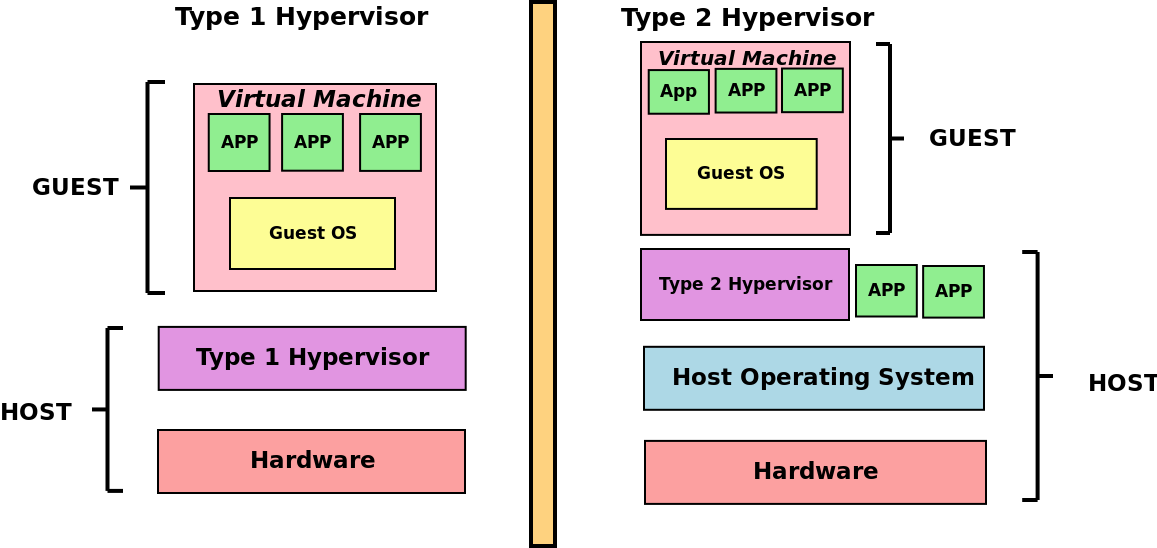
\includegraphics[width=10cm]{Hyper1vsHyper2}
	\caption{Type1 Hypervisor vs Type 2 Hypervisor}
	\label{Virtualization}
\end{figure}
%\newpage
\begin{itemize}
	\item \textbf{Type 1} hypervisor sits directly on hardware and manages virtual machines on top of it. It is also called bare-metal hypervisor. Examples of type 1 hypervisors are VMware vSphere/ESXi, Microsoft Windows Server 2012 Hyper-V, Citrix XenServer, Red Hat Enterprise Virtualization (RHEV) and open-source Kernel-based Virtual Machine (KVM) \cite{hypervisor2}.
	\item \textbf{Type 2} hypervisor runs on host operating system to manage virtual machines here hosted operating system provides hardware configuration.  VirtualBox and VMware
	Workstation are examples of type 2 hypervisors.
\end{itemize}
According to IBM, Type 1 hypervisors provide higher performance, availability, and security than Type 2 hypervisors.IBM recommends that Type 2 hypervisors be used mainly on client systems where efficiency is less critical or on systems where support for a broad range of I/O devices is important and can be provided by the host operating system \cite{searchservervirtualization}.
\\
Since bare-metal hypervisor has direct access to the hardware resources rather than going through
an operating system, it is considered to be more efficient than a hosted architecture and delivers greater scalability, robustness and performance \cite{hypervisor1}. 

\subsection{State of the Art Hypervisors\label{sec:comp}}
Over the past decade, virtualization technology has gone from small deployments to full blown IT infrastructure development. Technology makers have shifted their focus from operating systems with one-to-one relationships with hardware to virtualized approaches to shared resources among multiple operating systems on one hardware. When we talk about virtualization players in market, VMware is the first one which comes to our mind. Besides VMware, now other players like Citrix XenServer, Microsoft Hyper-V,Red Hat Enterprise Virtualization (RHEV), Oracle's Solaris Zones, LDoms and xVM, Amazon's Elastic Compute Cloud (EC2), Google Ganeti cluster virtual server management software tool and Virtual Bridges' VERDE product \cite{players} have entered this new market and are continuously developing innovation virtualization solutions to meet specific requirements of different industries. In 2011, Younge, Andrew J., et al. \cite{younge2011analysis} compared several virtualization technologies which is provided in Figure \ref{comparison}.
\begin{figure}[!htbp]
	\centering
	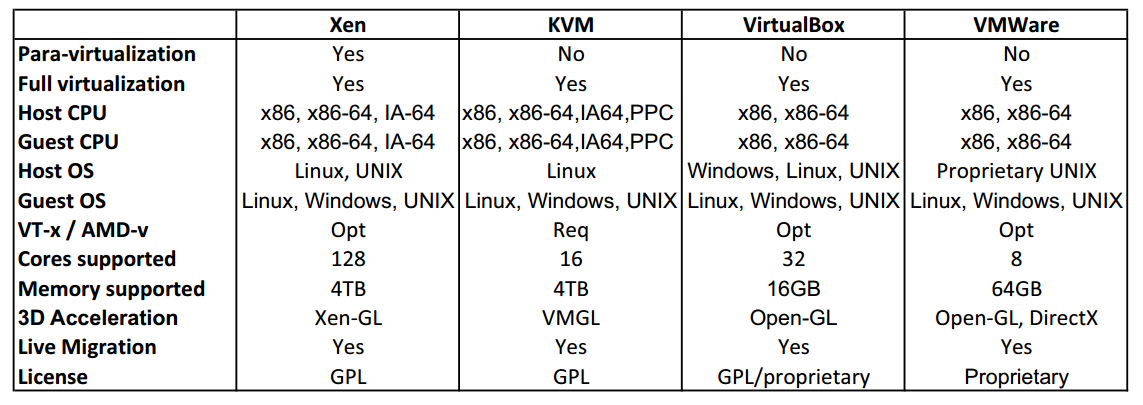
\includegraphics[width=10cm]{Comparison}
	\caption{A comparison chart between Xen, KVM, VirtualBox, and VMWare ESX. Adapted from from "Analysis of virtualization technologies for high performance computing environments" by Younge, Andrew J., et al, 2011, p11}
	\label{comparison}
\end{figure}

\section{Embedded Systems \label{sec:standard}}
Embedded systems are composed of simple devices used to perform small and dedicated functions with specific hardware and software constraints like low memory and efficient power usage, more battery life, smaller code footprint, smaller size and weight with reduced cost and reliability \cite{koopman1990design}. According to Steve Heath \cite{heath_2005}, an embedded system is a microprocessor-based system that is built to control a function or a range of dedicated functions and is not designed to be programmed by the end user in the same way as general purpose PC is. He had described several features of embedded systems which had led to the wide spread use of microprocessors in industry. Some of main features are as follows:
\begin{itemize}
	\item \textbf{Replacement of discrete logic circuits} to reduce the time and cost of developing new products by changing program code to process data in embedded systems.
	\item \textbf{Upgrading systems} by changing the software while keeping the hardware same thus reducing the cost of production and testing of software.
	\item \textbf{Providing easy maintenance upgrades} for adding new functionalities and resolving bugs by reprogramming the software without modifying the hardware.
	\item \textbf{Protecting intellectual property} by encapsulating the functionality of system by burning firmwares on chips making it harder to reverse engineer it.
\end{itemize}
In order to better understand embedded systems, we can look at differences from general purpose computers. General purpose computers are developed to run all types of general applications. However, embedded systems are designed for a fixed or a few number of dedicated functions. General purpose computers are reprogrammable by end users while embedded systems are not reprogrammable by end users. Embedded systems are smaller in size and run at fixed optimized speed for a specific purpose while general purpose computers are bigger in size with speed which does not need to be always predictable but faster is always better.
\\
\\
Embedded systems, once used only for single purpose time critical applications, are now becoming important for all devices used in our everyday life. Such devices are now able to run general purpose operating systems or application with little or no knowledge of hardware constraints. Although safety critical systems are far more restricted that so-called modern embedded systems, virtualization could bring advantages, by increasing their safety, reliability and security \cite{aguiar_hessel_2010}.

\subsection{Virtualization on Embedded Systems\label{sec:itu}}
 Adding a hypervisor to an embedded system adds flexibility and higher-level capabilities, morphing the embedded device into a new class of system \cite{ibm}. Embedded devices are ubiquitous and are major part of our lives today. Their common use is in real time applications with hardware and software constraints. But why there is a trend seen today to use these devices in virtualized systems. One of the reasons is that users now want to run applications developed originally for general purpose OSes and still desire to achieve real time responsiveness. There is where virtualization comes in handy. With virtualization, we can enable concurrent execution of real time OS (RTOS) and application OS(Windows, Linux etc) on same hardware. Another benefit will be security which can be achieved by encapsulating vulnerable application OS in a separate VM thus preventing access to the rest of the system.
 \\
 \\
 In a nutshell, there are many uses of deploying virtualization on embedded systems and with the development in multi-cores technology, we can expect innovative solutions in future embedded virtualized platforms. 

\subsection{ARM Embedded Platforms\label{sec:itu}}
Since the processor used in thesis is ARMv8 Cortex-A53, a brief introduction of ARM architecture in general and ARMv8 in specific along with its features will be provided in this section.
\subsubsection{Introduction to ARM Architecture\label{sec:arch}}
ARM, originally \textbf{Acorn RISC Machine}, later \textbf{Advanced RISC Machine}, is a family of reduced instruction set computing (RISC) architectures for computer processors, configured for various environments \cite{wikipedia_2017}. ARM has the following RISC architecture features \cite{ARM}:
\begin{itemize}
	\item A uniform register file load/store architecture, where data processing operates only on register contents, not directly on memory contents. 
	\item Simple addressing modes, where all load/store addresses are only determined from register contents and instruction fields.
\end{itemize}
With the increase in demands of new functionality and emerging market trends, ARM architecture has evolved over time. It has introduced the concept of \textbf{profiles} which define different versions of the architecture used for different types of processors which are aimed to to used in different market segments \cite{ARM}. Table \ref{tableARM} shows these different profiles of ARM architecture.
\begin{table}[!htbp]
\centering
\begin{tabular}[t]{|L{4cm} |L{8cm}|}
\hline
Profile & Description \\
\hline
Architecture (`A') profile  & Provides high performance and 
usually used in mobile and enterprise markets  \\
\hline
Real-Time (`R') profile & Provides real time performance and
 used in embedded applications for automotive and industrial control. \\
\hline
Microcontroller (`M') profile & Provides time critical and  real time performance for microcontroller market\\
\hline
\end{tabular}
\caption{Description of ARM profiles}
\label{tableARM}
\end{table}
ARM processors are basically used to achieve high-performance at lower cost with efficient power consumption.

\subsubsection{ARM processor modes and Registers\label{sec:processor_modes}}
There are two categories of ARM processor modes i.e. privileged  and non-privileged modes. Privileged mode is used to handle exceptions or to access system resources while non-privileged mode has restricted access to protected resources. Each processor mode uses a its own stack and a subset of registers. Table \ref{tab:modes} shows different processor modes supported by ARM architecture.
\begin{table}[!htbp]
	\centering
	\begin{tabular}[t]{|L{3cm} |L{8cm}|C{2cm}|}
		\hline
		\multicolumn{1}{|c|}{\textbf{Modes}}  &	\multicolumn{1}{|c|}{\textbf{Description}}    & 	\multicolumn{1}{|c|}{\textbf{Category }  }    \\ 
		\hline

		User                 & Normal program execution  & Privileged  \\\hline

		Fast interrupt (FIQ) & Handles fast interrupts  &     \\
        \cline{1-2}
		Interrupt (IRQ)      & Handles regular interrupts  &      \\
\cline{1-2}
		Supervisor           & Handles operating system functions. System enters into this mode when the power is applied.     &    \multirow{5}{*}{\centering Privileged}   \\
\cline{1-2}
		Abort                & Handles Data Aborts and Prefetch Aborts and helps to implement virtual memory        &      \\
\cline{1-2}
		System               & Handle operating systems function  in user mode and uses same registers as User mode    &      \\
\cline{1-2}
		Undefined            & Handles Undefined instructions with the support of software emulation of hardware co-processors &     \\
		\cline{1-2}
		Monitor & Provides support of switching between secure and  non-secure states available on processors with security extensions & \\
			\hline
	\end{tabular}
	\caption{Description of ARM processor modes}
	\label{tab:modes}
\end{table}
In all ARM processors, the following registers are available and accessible in
any processor mode \cite{arm_information_center}:
\begin{itemize}
	\item 13 general-purpose registers R0-R12
	\item 1 Stack Pointer (SP)
	\item 1 Link Register (LR)
	\item 1 Program Counter (PC)
	\item 1 Application Program Status Register (APSR)
\end{itemize}
ARM processor has total of 37 registers (40 with security extension implementations) arranged in partially overlapping banks which help to context switch rapidly. Figure \ref{ARM_Registers} shows the organization of general purpose registers of different ARM processor modes.


\begin{figure}[!htbp]
	\centering
	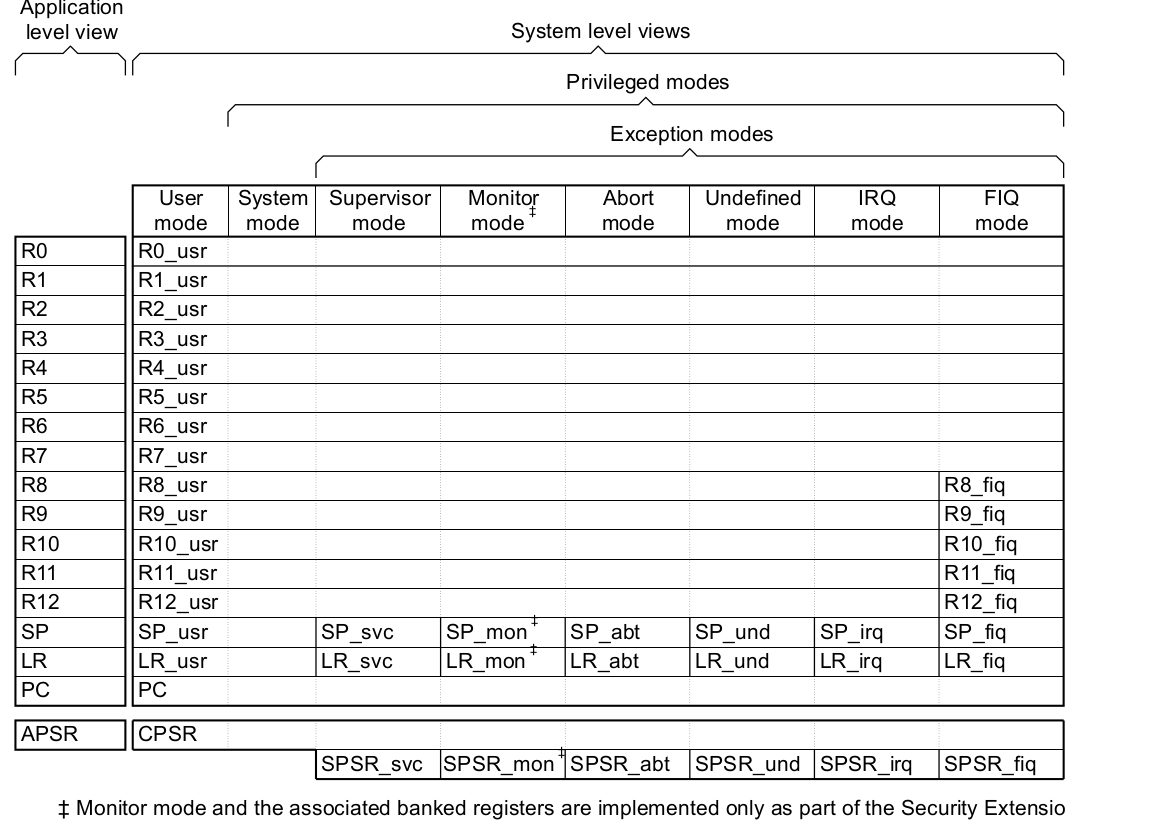
\includegraphics[width=10cm]{ARM_Registers}
	\caption{Organization of ARM registers for different processor modes. Taken from \cite{arm_information_center}}
	\label{Virtualization}
\end{figure}
\subsection{ARMv8-A Architecture\label{sec:armv8}}
The basic feature of ARMv8 architecture is that it supports both 32-bit (AArch32) and 64-bit (AArch64) execution states.For AArch64 state, addresses are placed in 64-bit registers and instructions can use 64-bit registers for processing while on the other hand, AArch32 allows instructions to use 32-bit registers  and addresses are placed in 32-bit registers \cite{armv8}. For this thesis, AArch64 execution state has been used which supports up to four Exception levels, EL0 - EL3 and has 64-bit virtual addressing. Table \ref{exeception_model} shows the description of exception model levels.
\begin{table}[!htbp]
	\centering
	\begin{tabular}[t]{|L{4cm} |L{8cm}|}
		\hline
		Exception Level & Description \\
		\hline
		 EL0 &  Applications\\
		\hline
		EL1 & OS kernel and associated privileged functions \\
		 \hline
		 EL2& Hypervisor  \\
		 \hline
		 EL3 &  Secure Monitor\\
		 \hline
	\end{tabular}
	\caption{Description of ARMv8 Exception Model Levels}
	\label{exeception_model}
\end{table}
The Cortex-A53 processor is a mid-range, low-power processor that implements the ARMv8-A
architecture with  Generic Interrupt Controller (GIC) v4 and ARM Generic Timer  \cite{cortexA53}.
\subsubsection{ARMv8-A Memory Management\label{sec:armv8_mem}}
Memory memory unit (MMU) is a hardware that performs virtual address to physical address mapping. It does this by controlling table walk hardware which accesses translation tables held in main memory.Transalation tables hold virtual to physical address mappings and memory attributes which are then loaded into the Translation Lookaside Buffer (TLB) when a location is accessed \cite{cortexA53}.
With MMU enabled in system, applications can run independently in their own virtual address space without having the knowledge of physical addresses used by hardware. Figure \ref{mmu} shows the MMU hardware in ARM architecture.
\begin{figure}[!htbp]
	\centering
	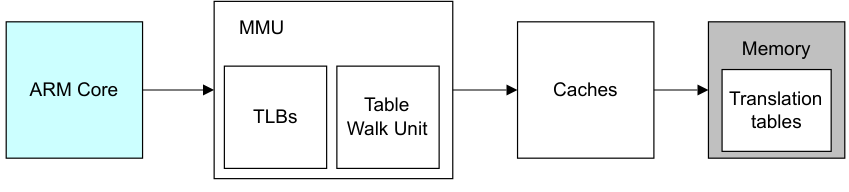
\includegraphics[width=10cm]{mmu}
	\caption{Organization of ARM registers for different processor modes. Taken from \cite{mmu}}
	\label{mmu}
\end{figure}

For ARMv8 hardware used in thesis, 48-bit virtual address with 4KB granule size has been used. Cortex-A53 processor uses a four level address lookup with 4KB page size. The 48-bit address has nine bits for each level of translation with the last 12 bits of original address defining the offset within the 4kB page size. Each level of translation lookup table has 512 entries.
Bits 47:39 of the Virtual Address index into the 512 entry L0 table. Each of these table entries spans a 512 GB range and points to an L1 table. Within that 512 entry L1 table, bits 38:30 are used as index to select an entry and each entry points to either a 1GB block or an L2 table. Bits 29:21 index into a 512 entry L2 table and each entry points to a 2MB block or next table level. At the last level, bits 20:12 index into a 512 entry L2 table and each entry points to a 4kB block \cite{translation}. Figure \ref{translation} shows the division of 48 bit address for four levels of translation lookup used for 4KB granule size by MMU.

\begin{figure}[!htbp]
	\centering
	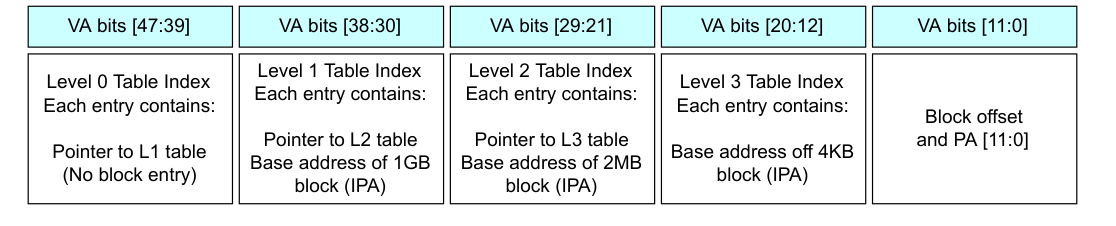
\includegraphics[width=10cm]{translation}
	\caption{48-bit address translation lookup for 4KB granule size on ARMv8 architecture. Taken from \cite{translation}}
	\label{translation}
\end{figure}


\subsection{Device Emulation on ARMv8-A Embedded Systems\label{sec:3gpp}}
ARMv8-A architecture supports virtualization by implementing EL2 execution state for running hypervisor. Hypervisor in EL2 state is responsible for running multiple guests in non-secure EL1 state. Each guest can run applications in non-secure EL0 state. Address translation occurs in two stages in case of running virtualized guest operating systems. Stage 1 translation converts virtual addresses to intermediate physical address (IPA) which is managed by Guest OS in EL1 state. Stage 2 translation converts IPA to physical address which is managed by hypervisor in EL2 state. These IPA are treated as actual physical addresses by Guest OS. ARM virtualization extensions has made generic timers and the GIC interrupt controller virtualization aware. Hence CPU, memory, interrupts and timers can be emulated using full hardware virtualization. However, for I/O devices, para-virtualized drivers could be used.\\
\\
On ARM architecture, device virtualization can be done using memory mapped devices. All reads/writes to devices gets trapped by hypervisor which should be capable of emulating device loads/stores. With ARM virtualization extensions, device virtualization has become more efficient. The main features of these extensions include  introduction of a new higher privileged Hypervisor execution mode than Supervisor mode, mechanisms to aid interrupt handling and the provision of a System MMU to aid memory management, supporting: multiple translation contexts for multiple DMA capable masters, two levels of address translation and hardware acceleration and abstraction \cite{ARM_VE}.
\\
Currently, on ARM virtualized systems, I/O devices can be emulated using either Type-1 or Type-2 hypervisors. Type 2 hypervisor allows to reuse guest OS code especially of device drivers for different types of hardware. However,Type 1 hypervisors requires device drivers to be reimplemented for a wide range of hardware support. Xen, a Type 1 hypervisor on ARM, has avoided this issue by implementing a minimal amount of hardware support directly in hypervisor and allows a special privileged guest called Domain-0 to perform I/O using existing device drivers on behalf of other non-privileged guests \cite{dall_li_lim_nieh_koloventzos_2016}.
\\
In short, ARMv8 architecture provides efficient virtualization as follows:
\begin{itemize}
	\item \textbf{CPU virtualization} with hypervisor in EL2 state configuring CPU to trap to sensitive and privileged instructions
	\item \textbf{Memory Virtualization} with hypervisor pointing to its own set of stage-2 translation tables for translating intermediate physical addresses to actual hardware addresses.
	\item \textbf{Interrupt Virtualization} with virtualization extensions support in ARM generic interrupt controller (GIC) to allow hypervisor to inject virtual interrupts to guests OSs which they can complete and acknowledge without being trapped in hypervisor.
	\item \textbf{Timer virtualization} by allowing guest VMs to configure virtual timer without trapping to hypervisor.
\end{itemize}

\section{Overview of Phidias Hypervisor \label{sec:summ}}
PHIDIAS, the Provable Hypervisor with Integrated Deployment Information and Allocated Structures, is the statically configured hypervisor developed by Dr.-Ing. Jan Nordholz at TU Berlin Telekom Innovation Laboratories with the faculty of Security in Telecommunications \cite{Jan}. It is second implementation of Principle of Staticity after Perikles which is being integrated in industrial automotive products at OpenSynergy \cite{opensynergy}.
\subsection{Principle of Staticity}
PHIDIAS is based on following Principle of Staticity which states that \\
\\
\textbf{\textit{Non-mandatory dynamic components of a hypervisor for an embedded system should be removed completely and if not possible, should reduce their dynamicity to generate a pure static and easily verifiable code by configuring the desired characteristics at compile time}}.\\
\\
The basic idea behind developing such minimal hypervisor is to remove all dynamic elements from it in order to ease provability and reduce runtime complexity as well as memory footprint. For certification of software to be used in safety critical applications, static analysis is widely used. If the behavior of software is constrained to be as static as possible with limited or no dynamic elements, it can be reliably proved and thus used in safety critical real time applications.
\subsection{Core Components of Minimal hypervisor implementation}
Memory requirements of virtual machines are defined at compile time which results in requested memory allocations
and alignment constraints to be verified and satisfied statically and assigning fixed physical
addresses to each of those allocations. All desired page tables, list of mapped memory ranges available to software and memory areas are finally compiled into the resultant bootable image. Virtual CPU interface, simulating full privileged and unprivileged register banks, is provided to run unmodified guests with hypervisor responsible for trapping and emulating certain sensitive instructions. This hypervisor is instantiated on each physical CPU for a multicore architecture running guest VMs on individual cores. It's scheduler is based on a simple single-priority round-robin policy. Dispatching of interrupts to VMs is done by a implementing a static interrupt dispatch table in read-only memory. Passing through an interrupt to a VM is done by using a second read only dispatch table which determines the target VM  for each interrupt line. PHIDIAS provides emulation of three basic hardware devices i.e. UART, timer, and interrupt controller. It does device emulation by implementing modifiable data structure to maintain the runtime state of emulated device and configuring guest physical memory ranges to which the device expects to respond to. Events and timers are implemented using event queue based on a single hardware timer with preallocation of timer events for signaling the end of time slice of virtual CPUs and timer events for each emulated timer device. Support of basic inter VM communication is also implemented using shared memory and signalling mechanism. This signalling mechanism is based on concept of capabilities. These capabilities are objects implemented internally in hypervisor that can be invoked to trigger desired actions e.g. triggering an interrupt to a target VM in case of inter VM communication. For systems without two stage address translation support in hardware, paravirtualized execution of virtual CPUs needs virtual translation lookaside buffer (VTLB).BVTLB implementation in PHIDIAS is based on two core components i.e. walker and pager. Walker component inspects effective guest page table in case of memory access fault and pager component adds hypervisor controlled two-stage translation of target address to the effective page table.
\subsection{Basic Structure of PHIDIAS}
The basic structure of PHIDIAS is shown in Figure \ref{Phidias_Structure}.

\begin{figure}[!htbp]
	\centering
	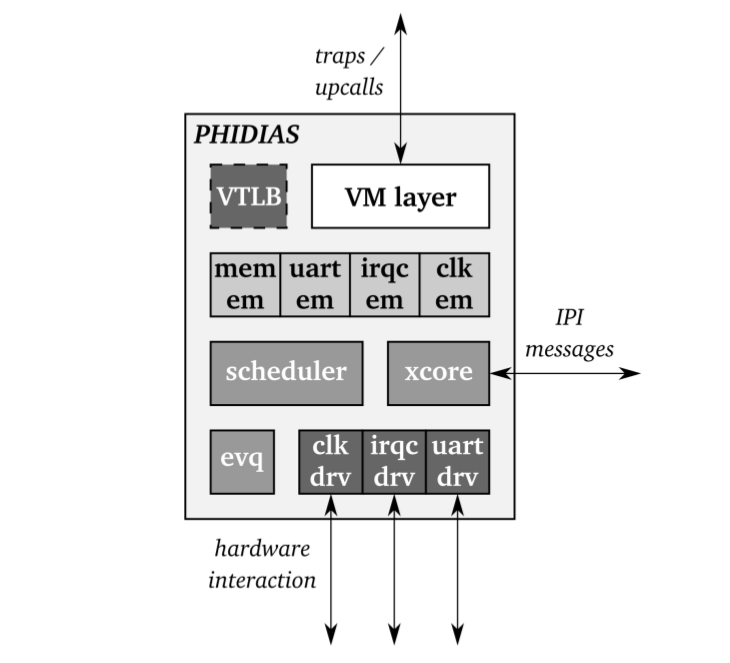
\includegraphics[width=10cm]{Phidias_Structure}
	\caption{Phidias Structure. Taken from \cite{Jan}}
	\label{Phidias_Structure}
\end{figure}

All mandatory components which are required for a hypervisor to function correctly are implemented in PHIDIAS. Following is a brief description of each of these basic components.\\
\\
\subsubsection{VM Layer}
VM Layer is responsible for performing world switch between guests and hypervisor. It performs upcall to enter into guests world and dispatches events to appropriate components for handling them. 
\subsubsection{Emulation Layer}
Emulation layer consists of minimal implementation of components necessary for hypervisor to operate. It includes UART, clock, Interrupt controller and a generic memory emulation. Generic memory emulation is added to run unmodified platform-specific Linux kernels without breaking their device specific functionality. Device driver sends memory requests to expected addresses but gets zero on reads and writes are discarded.
\subsubsection{Scheduler and Xcore}
At the heart of PHIDIAS, there is a scheduler with simple single-priority round-robin policy and Xcore components for relaying interprocessor interrupts between different instances of hypervisor and triggering interrupt capabilities.
\subsubsection{Event Queue and Drivers for emulation}
There is an event queue which is responsible for keeping track of programmed timer events and emulation drivers for minimal functionality is also present.

\subsection{Static Configuration and Final Image}
PHIDIAS is a static hypervisor which is built using a modifiable scenario specific configuration through an XML based compile time utility called Schism, the “Static Configurator for Hypervisor-Integrated Scenario
Metadata”. There are two types of configuration elements i.e. Hypervisor configuration and VM specific configuration elements.
\subsubsection{Hypervisor Configuration Elements}
\begin{itemize}
	\item Selection of CPU architecture and target platform SoC
	\item Physical and virtual Hypervisor base load address
	\item Selection of drivers for hardware devices and for the required emulation devices
\end{itemize}
\subsubsection{VM specific Configuration Elements}
\begin{itemize}
	\item Number of virtual CPUs per guest
	\item memory configuration per guest
	\item List of capabilities of each VM
	\item Assignments of pass-through interrupts to VMs
	\item Types, parameters, and corresponding emulated memory for selected emulated devices
\end{itemize}

